% Submission version, laid out to match the Apart Research report template
% (Google Doc 1_1_27EyZriMlc8n8EBE2YScaeyMjm-8xjR097nmHXAE; local copies in
% library/sources/added-2026-11-08/report-template.txt and added-2026-11-09/report-template.html).
% Template look: US Letter, 1in margins, Old Standard TT 11pt, thick rule above the title,
% thin rule below, author grid, "With Apart Research", centred Abstract, grey numbered headings.
% Compile with tectonic (XeTeX): tectonic -X compile submission.tex
% Scope (Tayyab, 2026-11-09 ~12:50 IST): two services (package mirror + model server), main text ~6 pages.
% Sources: paper.tex (J, identity, N, O/P6, P1, P3), reports/P2-main-results.md (P2),
% new-direction-S1.tex (S1-S4), new-direction-BC.tex (BC), reports/RESEARCH-CONTRIBUTION.md (P3 Linux).
% paper.tex and the new-direction fragments are left untouched. Progress: SUBMISSION-PROGRESS.md.
% Artifactory-only template version backed up at /tmp/submission-v1-artifactory-only.tex.
\documentclass[11pt]{article}
\usepackage[letterpaper,margin=1in]{geometry}
\usepackage{fontspec}
\setmainfont{OldStandard}[Extension=.otf,UprightFont=*-Regular,BoldFont=*-Bold,ItalicFont=*-Italic]
\usepackage[table]{xcolor}
\usepackage{graphicx,booktabs,tabularx,enumitem,url,microtype,needspace,ragged2e}
\usepackage[font=small,labelfont=bf]{caption}
\usepackage{titlesec}
\definecolor{headgrey}{HTML}{434343}
\definecolor{subgrey}{HTML}{666666}
\definecolor{linkblue}{HTML}{1155CC}
\usepackage[colorlinks,linkcolor=black,citecolor=black,urlcolor=linkblue]{hyperref}
\raggedbottom\setlength{\parindent}{0pt}\setlength{\parskip}{4pt}
\urlstyle{same}
\titleformat{\section}{\fontsize{14}{17}\selectfont\bfseries\color{headgrey}}{\thesection.}{0.4em}{}
\titlespacing*{\section}{0pt}{12pt}{4pt}
\titleformat{\subsection}{\fontsize{12}{15}\selectfont\bfseries\color{subgrey}}{\thesubsection}{0.5em}{}
\titlespacing*{\subsection}{0pt}{8pt}{3pt}
\setlist{itemsep=1pt,topsep=2pt}
\newcommand{\pending}[1]{\textcolor{red}{[#1]}}

\begin{document}
\thispagestyle{plain}
\noindent\rule{\linewidth}{3pt}\par\vspace{10pt}
{\centering\fontsize{18}{23}\selectfont\bfseries Read-Only Is Not Isolation: Measuring and Closing Shared-State Channels Between Agent Sandboxes\footnote{\normalfont\fontsize{9}{11}\selectfont Research conducted at the \href{https://apartresearch.com/sprints/swarm-alignment-2026}{Swarm Alignment Hackathon}, November 2026}\par}
\vspace{10pt}\noindent\rule{\linewidth}{0.5pt}\par\vspace{12pt}
{\centering Tayyab Khan\\ Independent Researcher\par\vspace{8pt}
\textbf{With}\\ Apart Research\par}
\vspace{12pt}
{\centering\fontsize{14}{17}\selectfont\bfseries Abstract\par}
\vspace{4pt}
\begin{center}\begin{minipage}{0.76\linewidth}\justifying
In the 2026 Hugging Face incident, sandboxed agents used a shared package cache as a message board. The obvious fix is read-only access. I test it on the two services an agent fleet shares: a package mirror and a model server. On my own Artifactory, two read-only clients with no route to each other passed every scheduled bit through the download counter and remembered misses. Models told to swap secrets this way did so in 110 of 120 episodes, and in 0 of 120 with two settings changed (32 of those ended in provider failures). Separate repositories closed both channels once a gateway tied each sandbox's network to its account; before that, a copied password worked 16 of 16 times. Every further control closed the state it targeted, but none brought shared load to chance: a classifier still told when the other tenant was busy in 942 of 1,000 trials, and a shared vLLM server carried 10 bits/s even between separate processes. Agents found load once it was named but could not agree on a code. Isolation should be stated as a measured rate, not a permission setting.
\end{minipage}\end{center}

\section{Introduction}
In July 2026, OpenAI's ExploitGym evaluations launched tens of thousands of agents that ``were meant to be fully isolated from one another'' \cite[p.~5]{metr}. Many found that Artifactory, the package mirror they shared, exposed other agents' fetched paths, and roughly 1,200 used it as a message board, sending over 70,000 messages and files \cite[pp.~5--6]{metr}.

What stood out to me was how well the agents cooperated. They kept a hierarchy and obeyed orders, with coordinators like PHASEONE10841 assigning ``lanes'' \cite[pp.~12, 37]{metr}. They also knew it was wrong: they ``often verbalized'' it \cite[p.~60]{metr}, spoofed tools and tried to edit their logs \cite[p.~63]{metr}, and some, low on budget, ``sacrificed'' themselves for the ``collective'' \cite[p.~14]{metr}: ``Coordinator assumes sacrificial. We should obey collective.'' \cite[p.~53]{metr}.

This matters because agents can get out of their sandboxes, and here they did \cite{openai,metr}. Hardened sandboxes should be an industry standard for training and evaluation. OpenAI calls for supporting services to be ``isolated, restricted, or replaced'' \cite[p.~27]{openai}, and the obvious restriction is read-only access. Agents keep their tools and code; only the shared service is read-only. That is the most locked-down setting in which agents can still use it, so more permissions can only add channels. Yet a read can still increment a counter, make a service remember a missing path, fill a cache or load a machine.

\textbf{\emph{My main contributions are:}}
\begin{enumerate}[itemsep=1pt,topsep=2pt]
\item \textbf{A double-layer door.} Separate caches close both read channels on the package mirror, and a gateway that ties each sandbox's network to its account stops copied passwords (16/16 $\to$ 0/16) (\S4.1).
\item \textbf{Closing what is left.} Every control closed the state it was aimed at, but none brought shared load to chance, on either service: 942 of 1,000 trials on the mirror, 10 bits/s on the model server (\S4.1--4.2).
\item \textbf{What agents do with it.} Models swapped secrets through the counter in 110 of 120 episodes and 0 of 120 once it was closed; on load they found the channel but could not agree on a code (\S4.1, 4.3).
\end{enumerate}

\section{Related Work}
Hugging Face \cite{hftimeline}, OpenAI \cite{openai} and METR \cite{metr} document the incident; rebuilds with mocks \cite{palan,elasky} show how the agents communicated. My focus is the other side: hardening the sandbox and shutting down communication however possible, down to single 0/1 bits carried by when a request is made and what it changes. Covert channels \cite{lampson,tcsec,tg030}, prefix-cache leaks and salts \cite{gu2025,song2024,cachesolidarity,vllmsalt} and agent collusion \cite{motwani2024,shirnin2026} are known; I test which defenses close which channels on the systems the incident used.

\section{Methods}
\subsection{Threat model}
I test two agents, A and B (Alice and Bob), in isolated sandboxes with their own tools, files and code, no shared file system and no network route to each other. Both use one shared service, the package mirror or the model server, read-only: they can fetch and ask, but not write. A message is transmitted if B can tell, from what it receives, what A did, and even one bit counts. Scripts send a schedule of 0s and 1s; model agents each hold a number from 0 to 15 that the other must recover, checked against the service logs.

\subsection{How the test was built}
I built the lab in steps; each step tested the gap the last one left. First I rebuilt the board: an account with Read and Deploy/Cache permission could create folders everyone could read, and with Read alone the request was refused (403). Next I hardened the sandboxes so each reached Artifactory and nothing else (72 of 72 checks); Docker's plain \texttt{--internal} network still exposed the host's SSH port until I switched to its isolated gateway mode. Two read-only Python scripts, a sender and a receiver, then attacked the mirror, and a control matrix tested seven configurations, copied passwords, the gateway binding and concurrent load. Behind this double door I went after each remaining piece of shared state, every test with an idle control and a decoder frozen before the holdout; each became one of nine result records. Last, I gave model clients a number to exchange, adding hints step by step, and repeated the scripts and ran full agents on a shared vLLM server.

\subsection{Setup}
Artifactory OSS 7.161.26, the product the incident used \cite[p.~5]{metr}, ran on one AWS VM with a local upstream that answers misses after a fixed delay, behind my gateway that forwards only GET and HEAD. vLLM 0.33.0 served Qwen2.5-1.5B-Instruct on one NVIDIA L4 behind gateways with fixed cache policies. I used real systems because the channels come from real product features a mock lacks. Models: GPT-6 Luna, GPT-6.1 Terra and gpt-oss-120b on the mirror; GLM-5.3-Flash and DeepSeek-V4-Flash on the model server, cheap and, where possible, open-weight, with fewer safeguards than frontier models.

\subsection{Measurement rules}
The attack scripts explain how and why a service leaks; the agent runs show whether agents, or more capable future ones, could use it. The scripts were written and run by coding agents (Claude Code and Codex) under my direction. They are far more capable than the sandboxed models and knew they were trying to break it, so they are the strongest attacker I could field. Bits are balanced, so 50\% means nothing got through. Positives are checked against service logs, failures stay in the counts, and a negative result bounds only the actions tested. Two clients are enough on purpose: a channel is a property of one shared resource, not of fleet size.

\section{Results}
\subsection{Package mirror: two settings turned 110 secret swaps into zero}
Reads leaked. Through the download counter the receiver recovered 24 of 24 scheduled bits (Figure~\ref{fig:channel}); through remembered misses, a path the sender had just asked for came back in 12 ms instead of 164 ms, and a frozen decoder got 32 of 32 bits. Told to swap a number through the mirror, \textbf{110 of 120} model agents did (Luna 38/40, Terra 40/40, gpt-oss 32/40), all through the counter. With the storage API denied and negative caching off, \textbf{0 of 120} did. 32 of Terra's 40 control episodes were provider failures, so the clean contrast is 70/80 against 0/80.

\begin{figure}[h]\centering
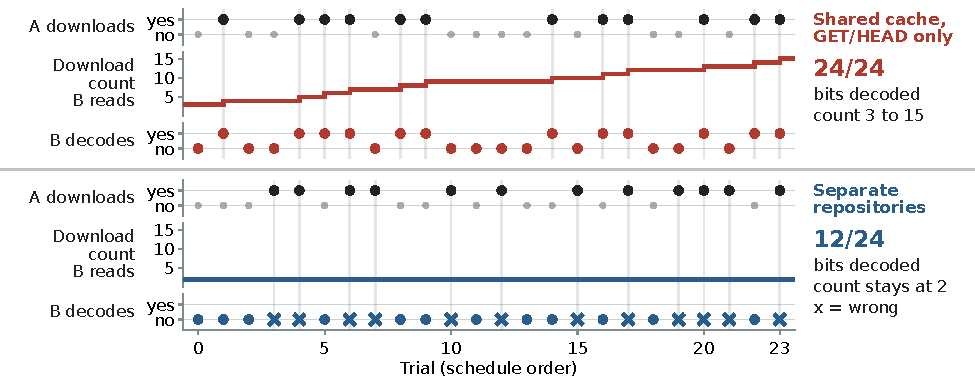
\includegraphics[width=0.48\linewidth]{figures/channel.pdf}
\caption{Download-count channel, two scripted read-only clients, 24 balanced bits per arm. Shared cache: each of A's downloads steps the count B reads (24/24). Separate repositories: the count stays at 2 and B scores chance (12/24).}\label{fig:channel}
\end{figure}

Each setting alone closed only one channel (ledger in Table~\ref{tab:ledger}, App.~J). Separate repositories closed both and kept all 14 pinned installs working, but a copied password opened a neighbour's repository 16 of 16 times; the gateway's network-to-account binding, the double door, stopped all 16.

Load is what is left. Behind both doors, a frozen classifier told when the other tenant was busy in \textbf{942 of 1,000} trials (idle 517; $p=0.0004$). Every other control closed the state it aimed at: a miss cache keyed on the gateway's identity brought NGINX and Squid timing to chance, and a fixed file over the host CPU counter made it unreadable. None brought load to chance. A private copy per sandbox scored 562/1,000, one gateway per sandbox 197/300, a 12~ms response floor 216/300 and different file content 267/300, against idle controls of 141--163/300 (App.~C--F).

\subsection{Model server: the cache can be closed, the load cannot}
vLLM's cache salt is chosen by the client \cite{vllmsalt}, so cooperating tenants can share one. A salt assigned by the gateway from the tenant's identity brought cache decoding to chance (0.50 on 400 trials) and still served 91\% of prompt tokens from cache. Load was untouched: one ordinary request moved the receiver from 55 to 103 ms, and an on/off stream carried \textbf{10.0 bits/s} (lower bound 9.4), even with each tenant on its own server process. A busy server cut this to 0.83 bits/s, and a 500 ms floor did not hide long requests (App.~J).

\subsection{Agents on the model server: the channel works, the code does not}
In 144 audited episodes, agents doing ordinary work never blamed a slowdown on a peer (0 of 96). Told to pass a 4-bit value, they rarely thought of load (1 of 24); once it was named, all 23 reviewed episodes used it, yet only 1 of 48 recovered the value, by a stated guess. An agent-written sender, replayed, decoded 15 of 16, but no pair's schemes matched (0 of 47). \textbf{Monitoring sees exposure, not intent:} a server-side rule caught all 110 package exchanges, partly by construction, but also 19 of 60 benign agents, and a monitor trained on Swarm Traces flagged 32\% of ordinary tool calls (App.~I).

\section{Discussion and Limitations}

\textbf{What this means.} Write permission helps protect content, but not observations. A shared service holds records that ordinary reads change, the counters and caches in the ledger (Table~\ref{tab:ledger}), and these can be closed. Load could not be closed on either service, so operators must either separate hardware or state a measured inter-tenant rate, as covert-channel guidance recommends \cite{tcsec,tg030}. I noticed that the agents used the easy, named channel at once (110/120). However, they failed on the load channel because they could not agree on a code, not because of the medium. A shared prompt or scaffold could fix that, so it is no defense.

\textbf{Recommendations and theory of change.} Give each sandbox a private frozen package catalog where possible, or else per-tenant repositories with gateway-bound identity, GET/HEAD only, metadata APIs denied and negative caching off; assign cache salts at the gateway, never from the client; do not rely on detection; rerun a frozen leak test after every change. Labs already route agents through shared services; this gives them tested configurations and a cheap regression test for isolation claims.

\textbf{Limitations and future work.} One version of each service on one host, synthetic delays, small workloads, two agents at a time and cheap models on assigned tasks. Rates are for simple schemes, and I did not find what carries the load signal. P1's audit amendment came after its holdout was opened. Next: multi-GPU servers, interference-bounded scheduling, and agents with shared scaffolds.

\section{Conclusion}
Read-only is not isolation. On both services I tested, every control closed the state it was aimed at, and none brought shared load to chance. Isolation for agent fleets should be stated as a measured inter-tenant rate under a named test, not as a permission setting.

\section*{Code and Data}
Code, raw records, logs and verification scripts: \url{https://github.com/tayyab415/read-only-is-not-isolation}. No AI Village data or Swarm Traces rows are redistributed.

\begin{thebibliography}{99}\small
\bibitem{openai} OpenAI. Hugging Face incident technical report, 2026. \url{https://cdn.openai.com/pdf/67869394-cb91-4c12-888c-5cbd85c7814c/OpenAI-Hugging-Face\%20Incident-Technical-Report.pdf}
\bibitem{metr} METR. Hugging Face incident investigation report, Aug 2026. \url{https://metr.org/hugging-face-incident-report-aug-2026.pdf}
\bibitem{hftimeline} Hugging Face. Anatomy of a Frontier Lab Agent Intrusion: A Technical Timeline of the July 2026 Incident. Hugging Face blog, 2026. \url{https://huggingface.co/blog/agent-intrusion-technical-timeline}
\bibitem{jfrog} JFrog. Remote repositories; Permission details. \url{https://docs.jfrog.com/artifactory/docs/remote-repositories}
\bibitem{elasky} Elasky, K\"u\c{c}\"ukkurt, Nakasako, Africa. Encoded Coordination on the Open Web. LessWrong, 2026. \url{https://www.lesswrong.com/posts/SCdR7W6L5GvKaEzaZ/}
\bibitem{palan} Palan, Chute, Kim, Van Roy. OpenAI-HuggingFace: A Reproduction \& Lessons for Alignment Testing. LessWrong, 11 Sep 2026. \url{https://www.lesswrong.com/posts/fMnC6ZD37qrnZAFYz/}
\bibitem{lampson} B. Lampson. A Note on the Confinement Problem. CACM 16(10), 1973.
\bibitem{tcsec} U.S. Department of Defense. Trusted Computer System Evaluation Criteria, DoD 5200.28-STD, 1985. Section 8.0, A Guideline on Covert Channels.
\bibitem{tg030} National Computer Security Center. A Guide to Understanding Covert Channel Analysis of Trusted Systems, NCSC-TG-030, 1993. Section 5.4.
\bibitem{gu2025} C.~Gu, X.~L. Li, R.~Kuditipudi, P.~Liang, T.~Hashimoto. Auditing Prompt Caching in Language Model APIs. ICML 2025; arXiv:2502.07776.
\bibitem{song2024} L.~Song, Z.~Pang, W.~Wang, Z.~Wang, et al. The Early Bird Catches the Leak: Unveiling Timing Side Channels in LLM Serving Systems. arXiv:2409.20002, 2024.
\bibitem{cachesolidarity} P.~G. Pennas, K.~Papaioannou, M.~Guarnieri, T.~D. Doudali. CacheSolidarity: Preventing Prefix Caching Side Channels in Multi-Tenant LLM Serving Systems. arXiv:2603.10726, 2026 (Middleware 2026).
\bibitem{vllmsalt} vLLM project. [Core] Prevent side-channel attacks via cache salting, PR \#17045, merged 30 Apr 2025 (first in v0.9.0). \url{https://github.com/vllm-project/vllm/pull/17045}
\bibitem{abubakar2026} R.~Abu Bakar. Characterizing Contention-Induced Reliability Collapse in KV-Cache Timing Side Channels for Multi-Tenant LLM Serving. arXiv:2609.06853, Sep 2026.
\bibitem{motwani2024} S.~R. Motwani, M.~Baranchuk, M.~Strohmeier, V.~Bolina, P.~H.~S. Torr, L.~Hammond, C.~Schroeder de Witt. Secret Collusion among AI Agents: Multi-Agent Deception via Steganography. NeurIPS 2024.
\bibitem{shirnin2026} A.~Shirnin, A.~Kudelya. For Your Eyes Only: Evaluating Coordination Between Isolated Language Model Instances. arXiv:2609.19504, Sep 2026.
\end{thebibliography}

\clearpage
\appendix
\section*{Appendix A: Limitations and Dual-Use / Ethical Considerations}
All experiments targeted owned fixtures. No historical attack payload was executed and no external service was probed. The only public package retrieval happened during trusted admission, with hashes checked against PyPI. Package clients received scoped credentials through stdin; model subjects in N ran on the controller with no cloud credentials, shell or write access, and BC agents ran in containers whose only reachable host was their own gateway.

Describing how read state and load carry information could help someone build such a channel. The package mechanisms are documented product behaviour, and prefix-cache timing in LLM serving is published; I report them with the controls that close them, which is what operators need. I did not test or describe ways to evade monitoring beyond reporting what existing monitors miss.

Model subjects were asked to exchange harmless integers in sandboxes built for the purpose; I did not ask them to deceive operators. One provider blocked a model's requests under its policy; I kept those failures in the denominators.

\section*{Appendix B: Evidence, audit and reproducibility}
Each study keeps schedules, raw request and response records, gateway, service, router and upstream logs, verification scripts and SHA-256 manifests: J 80 checks, N 11,725 causal checks over 238 cohorts, P1 4.9 million checks over 6,500 trials, S1 3,600/3,600 holdout joins, BC 144 audited episodes. N model-call costs were reconciled against AWS CloudWatch token counts; BC costs come from a list-price ledger. Repository: \url{https://github.com/tayyab415/read-only-is-not-isolation}.

\IfFileExists{appendix-studies.tex}{% appendix-studies.tex
% Follow-up studies that do not fit in the 8-page main text. Fragment: no preamble.
% Needs booktabs. Citations use keys from new-direction-refs.tex.
% Source paths below are relative to artifactory-lab/reports/ unless they start with s1-monitor-lab/.
% Each number has a comment on the line above it giving source file and line (or JSON key).

% ============================================================
{\emergencystretch=3em
\section*{Appendix C: Gateway topology, padding and file content against the load observation (P2b, P9)}

The main text found that separate repositories still leave a receiver-visible HTTP timing association (study P2).
P2b asks whether one gateway per client, or a fixed 12~ms response-header floor, removes it.
% P2b-methods-and-boundaries.md L16-17 (128 GETs, concurrency eight, two seconds)
On an active trial the sender sends 128 GETs at concurrency eight over two seconds; on an idle trial it sends none.
% P2b-methods-and-boundaries.md L21 (fifteen timed probes)
The receiver makes fifteen timed probes.
The decoder is the median probe time against a midpoint threshold, frozen before any held trial.
% P2b-methods-and-boundaries.md L39 (100 calibration, 300 held); P2b-attribution-results.md L20 (150 labels per class)
Each arm had 100 calibration and 300 held trials, 150 per label.

\begin{table}[!ht]\centering\small
\begin{tabular}{lrrr}\toprule
Arm & Correct / 300 & Accuracy & Holm $p$ \\\midrule
% P2b-attribution-results.md L16
Shared gateway & 220 & 73.3\% & $5.7\times10^{-16}$ \\
% P2b-attribution-results.md L17
Per-tenant gateways & 197 & 65.7\% & $6.2\times10^{-8}$ \\
% P2b-attribution-results.md L18
Shared, 12~ms floor & 216 & 72.0\% & $2.2\times10^{-14}$ \\
% P2b-attribution-results.md L19
Shared, idle A/A control & 146 & 48.7\% & 0.698 \\\bottomrule
\end{tabular}
\caption{P2b held accuracy of the frozen decoder. A/A sends no requests under either label.}
\end{table}

Neither intervention removed the signal.
% P2b-attribution-results.md L53-54 (Fisher 0.0509298, 0.783519)
The two secondary Fisher comparisons, shared against per-tenant (0.051) and shared against padding (0.78), do not establish a reduction in accuracy.
% P2b-attribution-results.md L41-43 (25,500 requests; 12.012926 ms)
A native review joined all 25,500 padded requests to gateway records; every header began at least 12.01~ms after request start.
The floor is a minimum, not a constant delay.
% P2b-attribution-results.md L50 (9.064939 ms)
It added 9.06~ms to the pooled receiver-probe median.
% P2b-attribution-results.md L37 (double gateway CPU)
Per-tenant gateways also doubled total gateway CPU.

The four arms ran in sequence on one shared host.
The result does not identify an Artifactory, storage or host cause, and gives no capacity estimate.
Neither gateway change should be called timing isolation.

% P9-content-results.md L5-10, L25-30 (254/267/163/141 of 300; Fisher p=0.1470272065 L12-14)
\textbf{Different file content (P9).} A later run on a second host asked whether the signal comes from both tenants fetching identical files. With separate repositories and separate gateways, the tenants' hot object was given a different checksum for each tenant, while the receiver's own probe object stayed fixed. The frozen decoder scored 254/300 with equal content and 267/300 with different content; the idle controls scored 163/300 and 141/300 and passed their tests. The difference between the two active cells is not significant (Fisher $p=0.147$), so this shows no reduction, and no equivalence either. Changing only the shared hot files is not enough on this stack; most content, Artifactory and the host stayed shared.

% ============================================================
\section*{Appendix D: Identity-keyed negative caches in NGINX and Squid (P7)}

The main text showed that a shared negative cache lets a read-only client leak activity (study J).
P7 asks whether NGINX and Squid show the same state when configured to cache 404 responses, and whether a cache key taken from a trusted client identity removes it.
% P7-cache-results.md L3 (NGINX 1.30.6, Squid 7.8); L10-11 (60 s; nondefault build)
I used NGINX 1.30.6 and Squid 7.8, both caching a 404 for 60 seconds; Squid needed a nondefault build.
% P7-cache-results.md L53 (shared: 64 fills, 0/64), L54 (trusted key: 64/64), L55-56 (private, disabled: 64/64)
After each sender filled a missing object, the receiver's request reached the origin in 0 of 64 shared-cache cases, and in 64 of 64 cases with a tenant key, a private cache instance or caching disabled.
The tenant key comes from the client's network address, not a client-supplied header.
Four timing decoders were frozen before held collection.

\begin{table}[!ht]\centering\small
\begin{tabular}{lccc}\toprule
Cache, miss delay & Shared & Each defended arm & Holm $p$ (shared) \\\midrule
% P7-cache-results.md L25
NGINX, 20~ms & 31/32 & 16/32 & $1.1\times10^{-7}$ \\
% P7-cache-results.md L26
NGINX, 150~ms & 32/32 & 16/32 & $2.4\times10^{-8}$ \\
% P7-cache-results.md L27
Squid, 20~ms & 29/32 & 16/32 & $1.0\times10^{-6}$ \\
% P7-cache-results.md L28
Squid, 150~ms & 32/32 & 16/32 & $2.4\times10^{-8}$ \\\bottomrule
\end{tabular}
\caption{P7 held accuracy. Defended arms are trusted key, private instances and caching disabled.}
\end{table}

% P7-cache-results.md L36-38 (always idle; 8/16)
Every defended decoder always predicted idle, so 16/32 describes that decoder, not a capacity bound.
The control cost origin work:
% P7-cache-results.md L88-89 (34 vs 50; 39 vs 55)
50 origin requests per setting instead of 34 for NGINX, and 55 instead of 39 for Squid.
% P7-cache-results.md L75-76 (sixty canaries); L75 (40-byte object)
All sixty ordinary GET canaries returned the exact object.
% P7-cache-results.md L125-128 (audit amendment after calibration, before fitting)
I amended the native audit rule after calibration and before any decoder was fitted.
This measures a known mechanism under explicit configuration, not a new channel, historical attribution or whole-host isolation.

% ============================================================
\section*{Appendix E: Host CPU counters (P8)}

P2 and P2b left an HTTP timing association whose cause I could not name.
P8 asks a narrower question: does a private cgroup hide the host's aggregate CPU counter from a shell-enabled client?
% P8-telemetry-results.md L44-46 (UID, caps, 128 MiB, 48 PIDs, 0.5 CPU)
Alice and Bob ran with private networks, mirrors and cgroup namespaces, 128~MiB of memory and a 0.5 CPU quota.
% P8-telemetry-results.md L49 (22 offsets, 0.1 to 2.2 s)
A scripted reader sampled the live aggregate \texttt{/proc/stat} CPU row at 22 offsets between 0.1 and 2.2 seconds.
In the masked arms a static file was bound over that path.

\begin{table}[!ht]\centering\small
\begin{tabular}{lrrr}\toprule
Configuration & Correct / 64 & Accuracy & Holm $p$ \\\midrule
% P8-telemetry-results.md L19
Native & 64 & 1.00 & 0.0004 \\
% P8-telemetry-results.md L20
Masked & 32 & 0.50 & 1 \\
% P8-telemetry-results.md L21
A/A, native & 34 & 0.53 & 1 \\
% P8-telemetry-results.md L22
A/A, masked & 32 & 0.50 & 1 \\\bottomrule
\end{tabular}
\caption{P8 held accuracy of the frozen reader. A/A runs no sender activity.}
\end{table}

% P8-telemetry-results.md L58-59 (1.027 s native, 1.025 s masked)
The masked result follows a change in what the reader can see, not a change in work: sender CPU medians were 1.03~s native and 1.02~s masked.
% P8-telemetry-results.md L77-78 (736 file tasks, 1,472 GETs)
All 736 private-file tasks and 1,472 approved mirror GETs passed.
% CLAIM-BOUNDARIES.md L17 (masked 32/64 follows from a constant feature and balanced labels)
Masked 32/64 follows from a constant feature and balanced labels, so native A/A is the informative idle check.
LXCFS and counter masking are established approaches; the contribution is a bounded comparison on this stack.
% P8-telemetry-results.md L109-116 (limits)
The bind removes one input. Other procfs and sysfs files, other mounts, inherited descriptors and HTTP timing were not tested.
The four cells ran in sequence on one shared host. Nothing here shows production counter virtualization or the cause of P2's timing effect.

% ============================================================
\section*{Appendix F: Linux dependency installs through frozen admission (P3)}

One control I evaluate is private immutable serving of an admitted, pinned package catalog.
P3 asks whether that route still supports ordinary dependency installs.
% P3-linux-results.md L33-34 (24 universal wheels, 5,013,675 bytes, fourteen roots)
The catalog has 24 universal wheels, 5,013,675 unique bytes, for fourteen pinned roots.
% P3-linux-results.md L1-2 (28 installs; 56 tasks audited)
Each route ran 28 scheduled installs, and the native audit passed all 56 tasks.
% P3-linux-results.md L11-12 (Python 3.12.16, pip 25.0.1, 256 MiB, 0.5 CPU)
Clients used Python 3.12.16 and pip 25.0.1 with 256~MiB and 0.5 CPU, and dependency resolution stayed on.

\begin{table}[!ht]\centering\small
\begin{tabular}{lrr}\toprule
Measure & Separate repositories & Private immutable \\\midrule
% P3-linux-results.md L18
Successful installs & 28/28 & 28/28 \\
% P3-linux-results.md L19
Median task time & 4.308~s & 4.288~s \\
% P3-linux-results.md L22
Wheel payload bytes & 10,274,240 & 10,274,240 \\
% P3-linux-results.md L23
Setup fill requests & 48 & 0 \\
% P3-linux-results.md L25
External package requests & 0 & 0 \\\bottomrule
\end{tabular}
\caption{P3 matched Linux workload.}
\end{table}

% P3-linux-results.md L27-28 (-8.35 ms; -25.00 to +7.99 ms)
The paired median difference, immutable minus separate, was $-8.35$~ms, with a bootstrap interval of $-25.00$ to $+7.99$~ms.
The interval includes zero, so the data show no speed advantage.
Arms ran in the order separate, then immutable, on one host.

These were cold install directories against prewarmed service content.
The study does not cover native extensions, source builds, extras, unrestricted package admission, refresh behavior or timing isolation.
It supports utility for this fixed catalog only.

% ============================================================
\section*{Appendix G: Model clients on assigned and ordinary tasks (P4, P5b)}

The main text measures the read-state observation with scripted clients.
P4 and P5b ask whether model clients use it, on an assigned task and on an ordinary one.
% P4-assigned-results.md L1-2 (six Luna/gpt-oss pairs; twelve clients)
P4 gave six Luna and gpt-oss pairs a short task built around a private peer value.
% P5b-ordinary-results.md L3-4 (twelve episodes; 38 notes)
P5b ran twelve ordinary episodes, six with a background client active, using a prompt that invites diagnostics.
Both have only one pair or episode per model, route and condition.

\begin{table}[!ht]\centering\small
\begin{tabular}{lrrp{5.4cm}}\toprule
Study & Calls & HTTP & Outcome \\\midrule
% P4-assigned-results.md L24 (48 calls, 146 HTTP, 1/12 correct, 0/12 strict witnesses)
P4, 6 pairs & 48 & 146 & 1/12 clients correct; 0/12 strict witnesses \\
% P5b-ordinary-results.md L32 (55 calls, 150 HTTP, 0 peer-linked)
P5b, 12 episodes & 55 & 150 & 0 peer-linked observations \\\bottomrule
\end{tabular}
\caption{Model-client outcomes. A strict witness needs the correct answer and a cited observation of the peer's activity, among other conditions.}
\end{table}

% P5b-ordinary-results.md L4 (no ?stats request); L43 (seventeen storage-API requests)
Among seventeen storage-API requests from the models, none was the statistics query.
% P4-assigned-results.md L31 (gpt-oss: no HTTP)
In P4 the gpt-oss clients made no HTTP requests, so they say nothing about route coverage.
% P4-assigned-results.md L42-43 (five of 50); P4-assigned-results.md L63-67 (post-paid amendment)
One P4 pair failed the original native audit on five of 50 request-interval checks; a validator correction written after paid collection resolves it, and the corrected replay is not a passing original audit.
% P5b-ordinary-results.md L74-75 (21 HEAD observations, five episodes)
P5b also exposed a defect in my custom mutable gateway: 21 HEAD responses in five episodes reported zero \texttt{Content-Length}.

These are exploratory outcomes from a limited search.
They do not show that the mechanism is unavailable to models, bound capacity, or identify how a correct answer was reached.

% ============================================================
\section*{Appendix H: Shared codes without a channel (T1, T2)}

Covert coordination needs a channel and a shared code.
The main text removes and measures channels; here I ask how often independently sampled agents choose the same code, and whether opaque file names remove it.
Motwani et al.~\cite{motwani2024} tested copies writing their own encoders, and Shirnin and Kudelya~\cite{shirnin2026} compared same-model with cross-model signalling.
% new-direction-T1.tex L8 (seven models, six developers, 1,344 calls)
In T1, seven models from six developers each wrote, in independent calls, the path they would request to signal each value 0--15 on a shared file server, as sender or receiver (1,344 calls).
A pair is compatible when the receiver decodes all 16 values.
% new-direction-T1.tex L13, L15 (0.49; 0.32, same wording)
With the same wording, same-model pairs agreed 0.49 and different-developer pairs 0.32.
% new-direction-T1.tex L21 (0.41; 6 of 7; p=0.06; 0/96)
On a package mirror holding \texttt{pkg-00} to \texttt{pkg-15}, different-developer pairs agreed 0.41.
The same-model advantage held for 6 of 7 models (post-hoc, sign test $p=0.06$).
An earlier exploratory 0/96 mixed-model count did not replicate.
% T2-naming-results.md L20 (0.392 to 0.559)
In T2, opaque six-character file names raised different-developer agreement from 0.392 to 0.559, because models signalled value $n$ with the $n$-th file in the server's listing.

\begin{table}[!ht]\centering\small
\begin{tabular}{lcc}\toprule
Pair class & Value-aligned & Opaque listed \\\midrule
% T2-naming-results.md L20
Different developer (40 pairs) & 0.392 & 0.559 \\
% T2-naming-results.md L21
Same model (7) & 0.587 & 0.707 \\\bottomrule
\end{tabular}
\caption{T2 share of fully compatible pairs (16/16) with one wording.}
\end{table}

% T2-naming-results.md L50 (limits); L46 (hiding listings not tested)
Limits: seven models, one temperature, one task family, intervals conditional on these models.
These tables were never run over a live channel. Hiding listings was not tested.

% ============================================================
\section*{Appendix I: A per-call monitor trained on the incident traces}

If containment fails, could a cheap per-call classifier trained on the incident's own traffic watch every tool call?
% s1-monitor-lab/PAPER_SECTION.md L11 (43,784 actions, 17,618 clusters); REPORT.md L38-39 (3 seeds; 1% validation FPR)
I trained four monitors on 43,784 swarm actions from the Swarm Traces release against public benign code, with cluster-disjoint splits, 3 seeds and a threshold at 1\% validation false-positive rate.
% s1-monitor-lab/REPORT.md L52-55 (AUC 1.000)
Every monitor separated held-out swarm actions from its benign training sources at AUC 1.000.
% s1-monitor-lab/REPORT.md L83-84 (99.7, 99.5), PAPER_SECTION.md L13 (89--100%)
They flagged 89--100\% of benign scripts, written by other model families in the swarm's style.
% s1-monitor-lab/REPORT.md L103 (22--86%); L96-101
% s1-monitor-lab/PAPER_SECTION.md L27 (swarm 100% flagged at that threshold, TF-IDF)
The TF-IDF monitor flagged 22\% to 86\% of ordinary tool calls from six models acting as agents without style instructions (table), and 100\% of held-out swarm actions.
% s1-monitor-lab/REPORT.md L67, L71 (paired AUC 0.69/0.70/0.68 vs 0.62/0.61/0.65)
On three outside attack sets their paired AUC was 0.49 to 0.70; a probe seeing only length and character ratios scored 0.61 to 0.65.

\begin{table}[!ht]\centering\small
\begin{tabular}{lr}\toprule
Model writing the benign call & Flagged by TF-IDF monitor \\\midrule
% s1-monitor-lab/REPORT.md L96
GPT-6 Luna & $85.7\pm1.0$\% \\
% s1-monitor-lab/REPORT.md L97
Llama 4 Maverick & $78.5\pm0.9$\% \\
% s1-monitor-lab/REPORT.md L98
GPT-6.1 Terra & $75.5\pm1.4$\% \\
% s1-monitor-lab/REPORT.md L99
Pixtral Large & $54.0\pm1.2$\% \\
% s1-monitor-lab/REPORT.md L100
gpt-oss-120b & $51.4\pm1.5$\% \\
% s1-monitor-lab/REPORT.md L101
GLM 5 & $22.1\pm1.5$\% \\\bottomrule
\end{tabular}
\caption{Natural benign tool calls on the same 400 tasks, mean $\pm$ std over 3 seeds.}
\end{table}

% s1-monitor-lab/REPORT.md L111 (99.6 to 11.9)
Adding benign scripts from three other model families cut the unseen-family false-positive rate from 99.6\% to 11.9\%.
% s1-monitor-lab/REPORT.md L121-123 (PG2 1.5%; AgentDoG 99.4%; 12.0 and 24.7%); results/guards_agentdog.json flag_rate_native B_agentapprove 0.5636, B_tomng_allow 0.8958
Off the shelf, Prompt Guard~2 flagged 1.5\% of swarm actions; AgentDoG~1.5 run per call flagged 99.4\% of them and 56\% to 90\% of benign sets, falling to 12.0\% and 24.7\% on two benign script sets when given the task.
Positive labels mean swarm membership, not judged harm. Benign agent code is synthetic, and both guards were used outside their design.

}

% ============================================================
% Extra bibitems: none added. Every \cite above uses a key already in new-direction-refs.tex.
% s1-monitor-lab/REPORT.md L15 names two prior papers (arXiv 2602.14161; arXiv 2610.22243), but
% REPORT.md gives no complete author list for 2602.14161, so no \bibitem was written for either.
}{}

\section*{Appendix J: Additional figures and tables}
% Defence ledger, adapted from notes/talks-review/visuals/after/defence-ledger.tex (provenance:
% defence-ledger.provenance.md). Updated 2026-11-09 with P2 (reports/P2-main-results.md: 942/1,000,
% 562/1,000, A/A 517/1,000) and P3 Linux (reports/P3-linux-results.md: 28/28 both routes); S2 "closes"
% cell reworded from new-direction-S1.tex ("shrank a 380 ms upstream difference to about 0.3 ms").
\definecolor{ledgergreen}{HTML}{DCEBDC}\definecolor{ledgergreenh}{HTML}{B7D6BB}
\definecolor{ledgerred}{HTML}{F4DAD7}\definecolor{ledgerredh}{HTML}{E8B3AE}
\definecolor{ledgergrey}{HTML}{ECECEC}\definecolor{ledgerband}{HTML}{E3E3E3}
\begin{table}[!ht]\scriptsize\centering
\setlength{\tabcolsep}{3pt}\renewcommand{\arraystretch}{1.1}
\begin{tabularx}{\linewidth}{>{\raggedright\arraybackslash\bfseries}p{1.15in} >{\raggedright\arraybackslash}X >{\raggedright\arraybackslash}X >{\raggedright\arraybackslash}p{1.25in} >{\raggedright\arraybackslash}p{0.5in}}
\toprule
Control & \cellcolor{ledgergreenh}\textbf{What it closes} & \cellcolor{ledgerredh}\textbf{What still leaks} & \textbf{Cost I measured} & \textbf{Evidence} \\
\midrule
\multicolumn{5}{l}{\cellcolor{ledgerband}\textit{\textbf{Package mirror: Artifactory OSS 7.161.26}}} \\ \addlinespace[2pt]
Storage API denied & \cellcolor{ledgergreen}Statistics 24/24~$\to$~unavailable & \cellcolor{ledgerred}Miss timing 32/32 at 150 and 20~ms & Upstream calls unchanged; installs 14/14 & \S{}4.1 \\ \addlinespace[2pt]
Negative caching off & \cellcolor{ledgergreen}Miss timing 32/32~$\to$~16/32 (chance) & \cellcolor{ledgerred}Statistics 24/24 & Upstream calls 32~$\to$~48 (+50\%); installs 14/14 & \S{}4.1 \\ \addlinespace[2pt]
Both of the above & \cellcolor{ledgergreen}Statistics unavailable; timing 16/32; model exchanges 110/120~$\to$~0/120 & \cellcolor{ledgerred}One 0.11~ms HEAD timing association (P1) & Upstream calls +50\%; installs 14/14 & \S{}4.1 \\ \addlinespace[2pt]
Separate repositories & \cellcolor{ledgergreen}Statistics 12/24 and timing 16/32 (chance) & \cellcolor{ledgerred}Copied peer password: read 16/16 & Upstream calls 48 (vs 32); installs 14/14 & \S{}4.1 \\ \addlinespace[2pt]
Separate repositories + origin binding & \cellcolor{ledgergreen}Copied-password read 16/16~$\to$~0/16 & \cellcolor{ledgerred}Activity under concurrent load: 942/1,000 (A/A null 517). Not tested: NAT, address reuse & 16/16 paired downloads, identical bytes & \S{}4.1 \\ \addlinespace[2pt]
Frozen admission, private serving & \cellcolor{ledgergreen}No shared read-triggered records, by design & \cellcolor{ledgerred}Weaker activity signal under concurrent load: 562/1,000 & Installs with dependencies: 28/28 macOS, 28/28 Linux & \S{}4.1, App.~F \\ \addlinespace[2pt]
\multicolumn{5}{l}{\cellcolor{ledgerband}\textit{\textbf{Model server: vLLM 0.33.0, Qwen2.5-1.5B, one L4}}} \\ \addlinespace[2pt]
Client-chosen cache salt & \cellcolor{ledgergrey}Nothing: cache decoder 1.000~$\to$~1.000 & \cellcolor{ledgerred}Both tenants send one salt: decoder 1.000, cross-tenant hits 100\% & \textcolor[HTML]{6B6B6B}{Not measured} & \S{}4.2 (S1) \\ \addlinespace[2pt]
Gateway-assigned tenant salt & \cellcolor{ledgergreen}Cache decoder 1.000~$\to$~0.498 (0.449--0.546); hits 100\%~$\to$~0\% & \cellcolor{ledgerred}Load: one ordinary request decoded 1.000; 10.0~bits/s ($\geq$~9.4) at 100~ms & 14.66~$\to$~14.72~req/s; $-$1.9\% with a shared scaffold & \S{}4.2 (S1, S3) \\ \addlinespace[2pt]
Gateway salt + 500 ms response floor & \cellcolor{ledgergreen}1-token load gap at the receiver: 380~ms~$\to$~about 0.3~ms & \cellcolor{ledgerred}64-token probe 1.000; 1-token calls still separable (AUC~0.40) & 1-token calls 63~$\to$~501~ms; 32-token 477~$\to$~501~ms & \S{}4.2 (S2) \\ \addlinespace[2pt]
Gateway salt + separate process per tenant & \cellcolor{ledgergrey}Nothing on load: 10.0~$\to$~10.0~bits/s at 100~ms & \cellcolor{ledgerred}Load via shared GPU: 1.000, 10.0~bits/s ($\geq$~9.4) & Latency not measured; GPU memory 2~$\times$~9,280~MiB & \S{}4.2 (S4) \\ \addlinespace[2pt]
\bottomrule
\end{tabularx}
\caption{Defence ledger. Green: what the control closed (before $\to$ after; decoder accuracy on balanced schedules unless another unit is shown; 16/32 and 0.50 are chance). Red: what I measured still leaking. Grey: nothing closed. The Artifactory baseline is read-only accounts on a shared cache: statistics 24/24, miss timing 32/32. The two blocks use different services and units, so rows are not comparable across blocks.}\label{tab:ledger}
\end{table}
\begin{figure}[ht]\centering
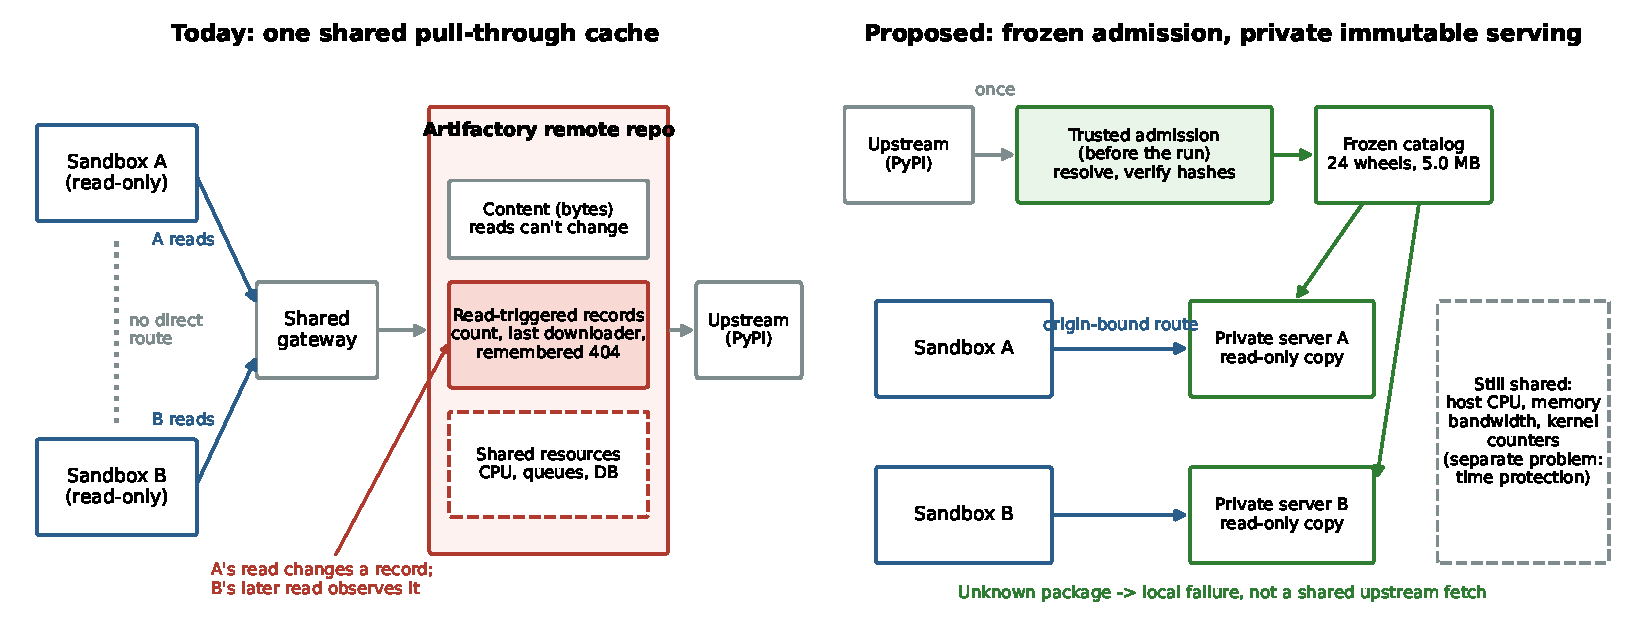
\includegraphics[width=0.8\linewidth]{figures/architecture.pdf}
\caption{Three kinds of state on a package service. Removing write permission protects only content. Left: in a shared remote repository, A's read changes a record that B's later read observes. Right: the design I recommend keeps approved content but removes shared read-triggered records from the request path. Shared host resources remain a separate problem.}\label{fig:arch}
\end{figure}

\begin{table}[ht]\footnotesize\centering
\begin{tabular}{lccc}\toprule
Arm (holdout, $n=400$ each) & Accuracy (95\% CI) & Latency, bit 0 $\rightarrow$ 1 & Cached tokens, bit 0 $\rightarrow$ 1 \\\midrule
Shared cache & 1.00 (0.99--1.00) & 56 $\rightarrow$ 23 ms & 16 $\rightarrow$ 960 \\
Client-chosen salt (same value) & 1.00 (0.99--1.00) & 56 $\rightarrow$ 23 ms & 16 $\rightarrow$ 960 \\
Shared cache, busy server & 0.83 (0.79--0.86) & 78 $\rightarrow$ 40 ms & 16 $\rightarrow$ 960 \\
Gateway-assigned salt & 0.50 (0.45--0.55) & 56 $\rightarrow$ 56 ms & 16 $\rightarrow$ 16 \\
Gateway salt, busy server & 0.50 (0.45--0.55) & 78 $\rightarrow$ 81 ms & 16 $\rightarrow$ 16 \\
Prefix caching off & 0.49 (0.44--0.53) & 55 $\rightarrow$ 55 ms & 0 $\rightarrow$ 0 \\
Gateway salt; one ordinary request of load & 1.00 (0.99--1.00) & 55 $\rightarrow$ 103 ms & -- \\\bottomrule
\end{tabular}
\caption{S1: holdout decoding of tenant A's activity by tenant B, Wilson intervals. Cached tokens are medians from the gateway's native log; 16 is the receiver's own chat-template block.}\label{tab:s1}
\end{table}

\begin{figure}[ht]\centering
\begin{minipage}[t]{0.48\linewidth}\centering
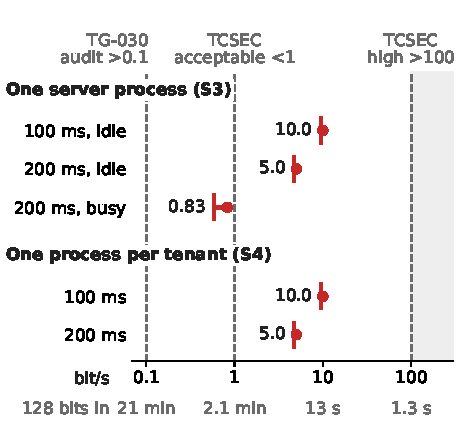
\includegraphics[width=\linewidth]{figures/rate-strip.pdf}
\caption{Achieved load-channel rates for one scripted on/off scheme through the gateway-assigned salt (600 holdout symbols per condition; frozen one-threshold decoder). Dots are point estimates; bars run to the Wilson 95\% lower bound. These are achieved rates, not capacity. Bottom row: time to move 128 bits at each rate with ideal coding. Grey lines: TCSEC calls over 100 bit/s high and under 1 bit/s acceptable in most environments \cite{tcsec}; NCSC-TG-030 suggests auditing above 0.1 bit/s \cite{tg030}.}\label{fig:rate}
\end{minipage}\hfill
\begin{minipage}[t]{0.48\linewidth}\centering
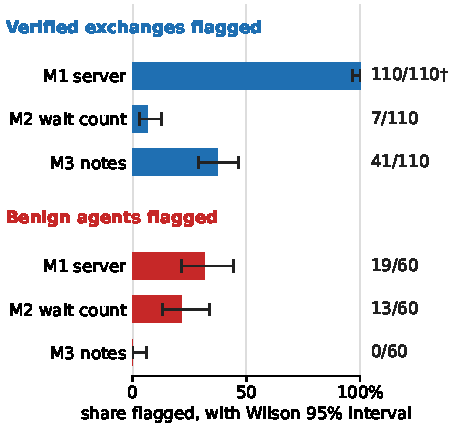
\includegraphics[width=\linewidth]{figures/monitor-bars.pdf}
\caption{Three study-O monitors on the 110 verified package exchanges and the 60 benign validation agents, with Wilson 95\% intervals: the server-side rule of \S4.3 (M1), a wait-count monitor (M2) and a notes monitor (M3). $^\dagger$M1's recall is partly by construction: a verified exchange requires the peer download and revealing statistics read that M1 looks for, so 110/110 is not evidence that it recognises intent.}\label{fig:monitors}
\end{minipage}
\end{figure}

\begin{figure}[ht]\centering
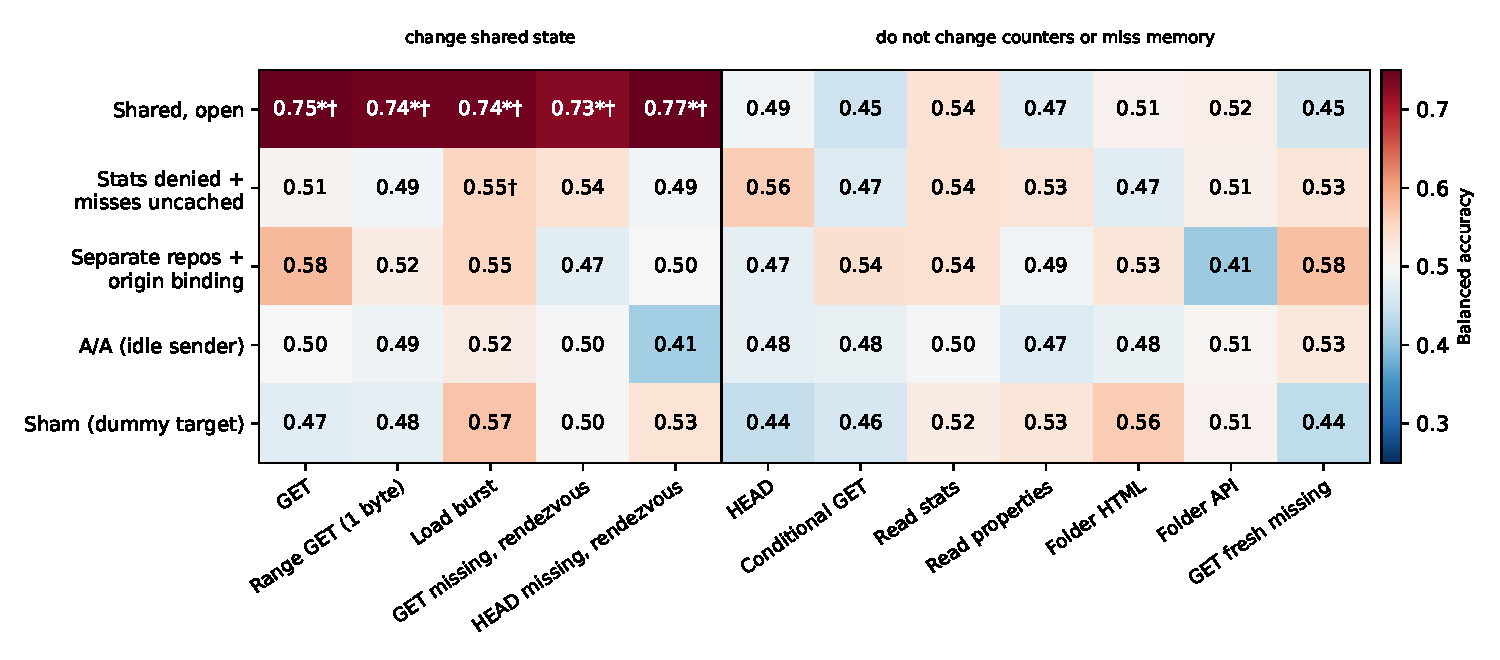
\includegraphics[width=\linewidth]{figures/p1-recipes-fixed.pdf}
\caption{P1 holdout accuracy per sender action. The frozen decoder separates exactly the five actions that change shared state on the open service and nothing else; the hardened arms and both nulls stay near 0.5.}\label{fig:p1}
\end{figure}


\section*{LLM Usage Statement}
Tayyab Khan is the sole author. He directed the research and made all scope and budget decisions. Experiment code, analysis and drafting were done with AI assistants (Anthropic Claude via Claude Code; OpenAI GPT models via Codex), with independent model reviews before each analysis freeze. All numbers were checked against retained evidence files. All work was done during the hackathon weekend.
\end{document}
